\Exhibit{FceDemo}{%
    Screenshot of Apache Beam Playground, an application that uses Flutter Code Editor%
}

This screenshot shows Apache Beam Playground web application developed by Akvelon
for \Asf.
It is a sophisticated application with multiple functions.
In the central part, the code editor is that `Flutter Code Editor',
a product by Akvelon that can be reused in different applications.

On this screenshot:

\begin{itemize}
    \item Lines 2--17, 19--31, and 34--58 are folded so as not to distract the programmer.
    \item Autocompletion is suggesting a word as it is typed.
    \item Cross marks show errors.
    \item One of the cross marks shows the error message when hovered over.
\end{itemize}

The unique feature of Flutter Code Editor is that this app and all of the features listed above run in a browser
and can also be potentially turned into native mobile apps for both iOS and Android effortlessly.

\begin{center}
    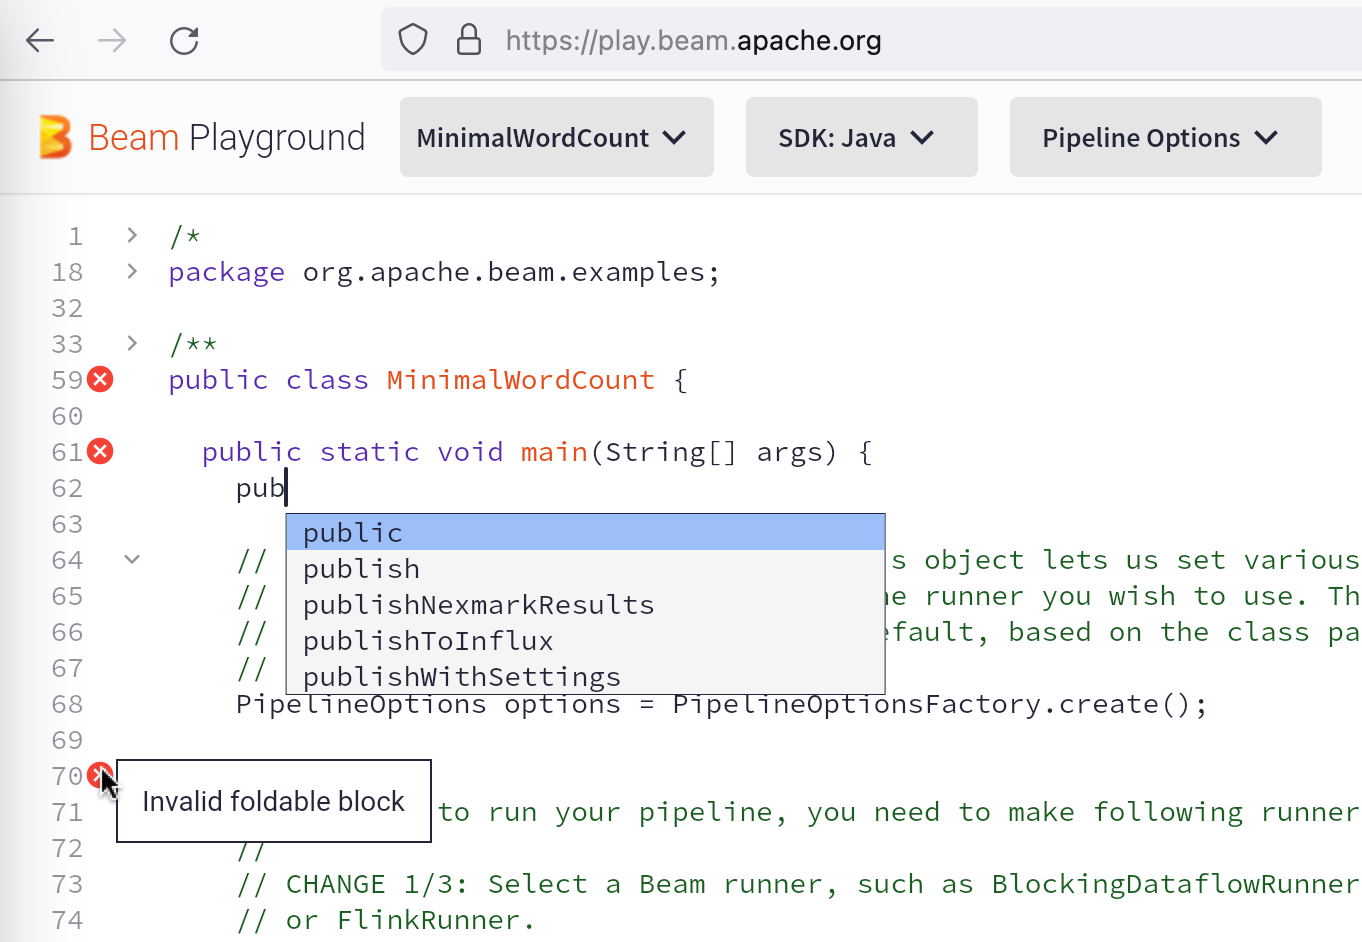
\includegraphics[width=30em]{demo}
\end{center}

\pagebreak
